\chapter{}

\section{App}
The demo app is inspired by the tutorial \href{https://developer.android.com/courses/android-basics-compose/unit-1}{Unit 1: Your first Android App} on the Android Studio website. It features a background image and a content part devised sections using the \textsl{Column} and\textsl{Box} environment for composables. We present a name in coloured letters with a circular profile picture beneath. Further down we see a small bio section and a contact email address.
In Fig. \ref{fig:app_screen} we see screenshots of the app screen in both the built-in previewer and the emulator of Android Studio.


\begin{figure}
	\centering
	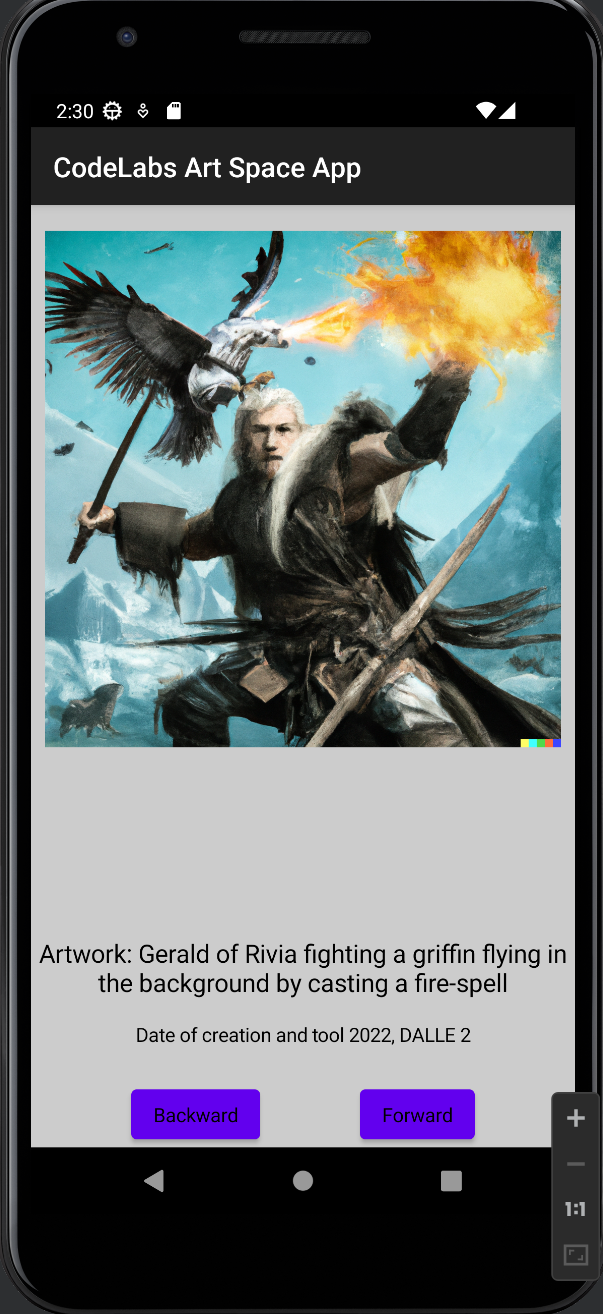
\includegraphics[width=.3\linewidth]{figures/app_screenshot_1.png}
	\caption{Screenshot of app screen in preview windows of Android Studio}
	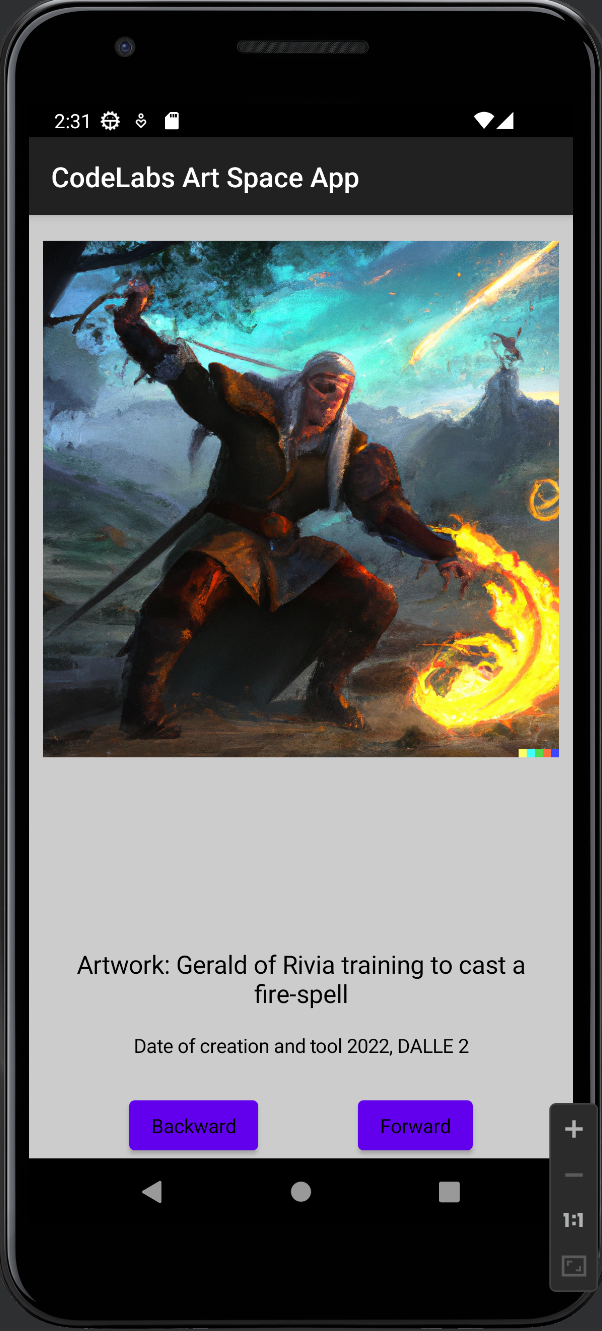
\includegraphics[width=.3\linewidth]{figures/app_screenshot_2.png}
	\caption{Screenshot of app screen in emulator of Android Studio}
	\label{fig:app_screen}
\end{figure}

\section{CodeLab: A report on usability}
% Basic examples :Hello World, Declare variables/functions, retaurn values --> beginner friendly, maybe a bit too easy for expirienced programmers?
% Advanced Tutorial: Graphical design similar to HTML, programming similar-ish to java o other high level languages
In my opinion, the CodeLab tutorial are well designed for the most part. They start with basic examples and get more advanced step by step. The choice to first introduce the Kotlin language seems logical to me. Though it lacks in-depth sections for more advanced programmers.

The section on how to use Android Studio seems to follow the same philosophy by starting at the beginning with the installation and moving on to usage and setup of functions such as the built-in emulator. It provides the basic knowledge on how to use Android Studio. Though, again, a bit more in-depth knowledge or examples for workflow integration could be added to these tutorials.

Last but not least, the design and layout tutorial. They introduce the \textsl{Jetpack Compose} system that helps with a standardized way on how to design the screen of any app. It has some similarities to \texttt{HTML} and \texttt{CSS} as we can use common modifiers to apply certain effects or alignments to our elements.
The tutorial does a fairly good job explaining the possible elements, but it would have been nice of them to provide code blocks for every feature they introduce to enable the user to play around with it. Furthermore, we think that some explanations are too complicated, since the other parts of the tutorial were targeting a fairly inexperienced audience.

In total we believe these tutorials to provide a solid foundation to new android developers. As we pointed out, there is still a lot of room to improve, but the general direction is definitely right.

